\subsection{Scaling Up the Training Corpus}\label{sec:exps_dolma}

\begin{table*}[t]
\caption{Zero-shot evaluation accuracy on downstream tasks. Models with f-gram embedding layers show clear improvements over the baseline models.  }
\label{table:dolma_downstream}
\centering
\setlength{\tabcolsep}{5pt}
\resizebox{1.0\linewidth}{!}{
\begin{tabular}{l|cccccc|c}
\toprule
\textbf{Model} & \textbf{PIQA} & \textbf{HellaSwag} & \textbf{ARC-E} & \textbf{ARC-C} & \textbf{CSQA} & \textbf{MMLU} & \textbf{Avg.} \\
\midrule
OLMo-1B & 73.6 & 60.9 & 69.5 & 31.8 & 48.7 & 37.6 & 53.7 (+0) \\
%\midrule
OLMo-1.9B & 75.3 & 65.9 & 74.2 & 36.8 & 49.7 & 38.6 & 56.8 (+3.1) \\
%\midrule
OLMo-1B + OE-12.8M \citep{huang2025over} & 73.7  & 62.7 & 70.3 & 32.1 & 49.9 & 37.8  & 54.4 (+0.7)  \\
%\midrule
OLMo-1B + 10M f-grams & 74.0 & 63.6 & 70.4 & 32.1 & 49.9 & 39.3 & 54.9 (+1.2) \\
%\midrule
OLMo-1.3B + 10M f-grams & 75.0 & 65.5 & 75.3 & 36.4 & 49.9 & 38.5 & 56.8 (+3.1) \\
%\midrule
OLMo-1B + 1B f-grams & 75.3 & 67.1 & 72.5 & 36.4 & 50.8 & 39.9 & 57.0 (+3.3) \\
\bottomrule
\end{tabular}
}
\end{table*}


After exploring several design choices for \SCONE, we now evaluate its performance in large-scale pretraining. Our implementation builds on the open-source OLMo codebase \citep{OLMo}, licensed under Apache 2.0. Additional implementation details are provided in \Cref{subsec:dolma_details}.

\textbf{Downstream Tasks.} We report zero-shot accuracy on six standard downstream benchmarks: MMLU-var, Hellaswag, ARC-Challenge, ARC-Easy, CommonsenseQA (CSQA), and PIQA. In the main text, we focus on presenting downstream accuracy results under our primary training setting. Additional results, including perplexity evaluations, training curves, and further \SCONE configurations under alternative settings, are provided in \Cref{subsec:more_exp_dolma}. Notably, perplexity trends closely correlate with downstream performance.

\textbf{Baselines.} We compare \SCONE against three baselines: OLMo-1B, OLMo-1.9B, and a concurrent method, the over-tokenized transformer \citep{huang2025over}. Model configurations for OLMo-1B and OLMo-1.9B are detailed in Appendix~\ref{subsec:dolma_details}. For the over-tokenized transformer, we adopt the best-performing OE-12.8M variant, which introduces an additional input embedding layer comprising 12.8M embedding vectors, applied on top of the OLMo-1B model. Further discussion of this method can be found in \Cref{sec:related_work}. All baseline models are trained for 1T tokens.

\textbf{SCONE Configuration.} We apply \SCONE with two f-gram embedding layer sizes: 10M and 1B f-grams, respectively. The cutoff frequencies are 21,956 for 10M f-grams and 70 for 1B f-grams. \SCONE is integrated into OLMo-1B and OLMo-1.3B models, with an $\Afgram$ model size of 1.8B parameters (matching the architecture of OLMo-1.9B but excluding the token embedding layer). Models equipped with \SCONE are trained for 500B tokens, half the number of tokens used by the baselines, to account for the additional training cost of the $\Afgram$ model and ensure comparable total training FLOPS. In \Cref{subsec:more_exp_dolma}, we also explore a smaller $\Afgram$ model of 0.6B parameters, where we observe consistent improvements.

\textbf{Results.} \Cref{table:dolma_downstream} presents the downstream accuracy results. Models with \SCONE demonstrate clear improvements over the baselines. Specifically, with 10M f-grams, OLMo-1.3B achieves parity with the OLMo-1.9B baseline while using approximately 32\% less inference FLOPS and accelerator memory. With 1B f-grams, OLMo-1B slightly outperforms the OLMo-1.9B baseline while requiring approximately 48\% less inference FLOPS and accelerator memory. Compared to the over-tokenized transformer, OLMo-1B + 10M f-grams surpasses OLMo-1B + OE-12.8M, which we attribute to the additional capacity introduced by the $\Afgram$ model during training.


\subsection{Space Usage and Query Latency}
\label{subsec:inference_cost}

We show that the latency of the f-gram embedding layer does not constitute a bottleneck during inference, and that system memory and solid-state storage are relatively inexpensive. In \cref{subsec:compute_resources}, we also provide a unified table summarizing the key metrics: (1) GPU memory, (2) CPU memory, (3) disk usage, and (4) FLOPS/latency for training and inference.

\begin{table} [h]
    \caption{Space usage of the f-gram embedding layer $\cF$, along with unit cost for memory and NVMe solid-state drives \citep{memory_disk_price}.}
\label{tbl:space}
\centering
\small
\renewcommand{\arraystretch}{1.2}
\begin{tabular}{ P{2.0cm}P{2.4cm}  P{2.4cm} }
 \toprule
  \# of \ngram{n}s       & System memory (GB) & Solid-state drive (GB)		 \\\midrule
$10^{7}$    &   41.4  &	  77.3 	\\
%\hline
$10^{8}$    &   413.6  &  766.8 	\\
%\hline
$10^{9}$    &   (does not fit)  &	7665.4 	\\\midrule
%\hline

Price (per GB) & $\sim$ 2 USD  & $\sim$ 0.1 USD  \\\bottomrule %\hline
\end{tabular} 
\end{table}

We experiment with $|\Vfgram|$ being 10M, 100M, and 1B with embedding dimension of $d = 2048$ and 16-bit precision per floating point value. Experiments were conducted on a workstation with 64 Intel Xeon CPU cores and 512 GB of memory. Space and latency were measured for both in-memory and on-disk storage. In memory, embeddings are stored as a single matrix with a hash dictionary mapping f-grams to indices, while on-disk storage uses the Lightning Memory-Mapped Database \citep{lmdb} to directly store f-gram and embedding pairs on NVMe solid-state drives.




\Cref{tbl:space} summarizes the space usage for both storage methods. In both cases, the space required increases linearly with the number of embedding vectors. 
The 10M and 100M f-gram embedding layers are able to fit within main memory, with the 10M layer requiring 41.4 GB. For on-disk storage, there is additional overhead as the same 10M layer occupies 77.3 GB storage.


\begin{figure}[t]
    \centering
    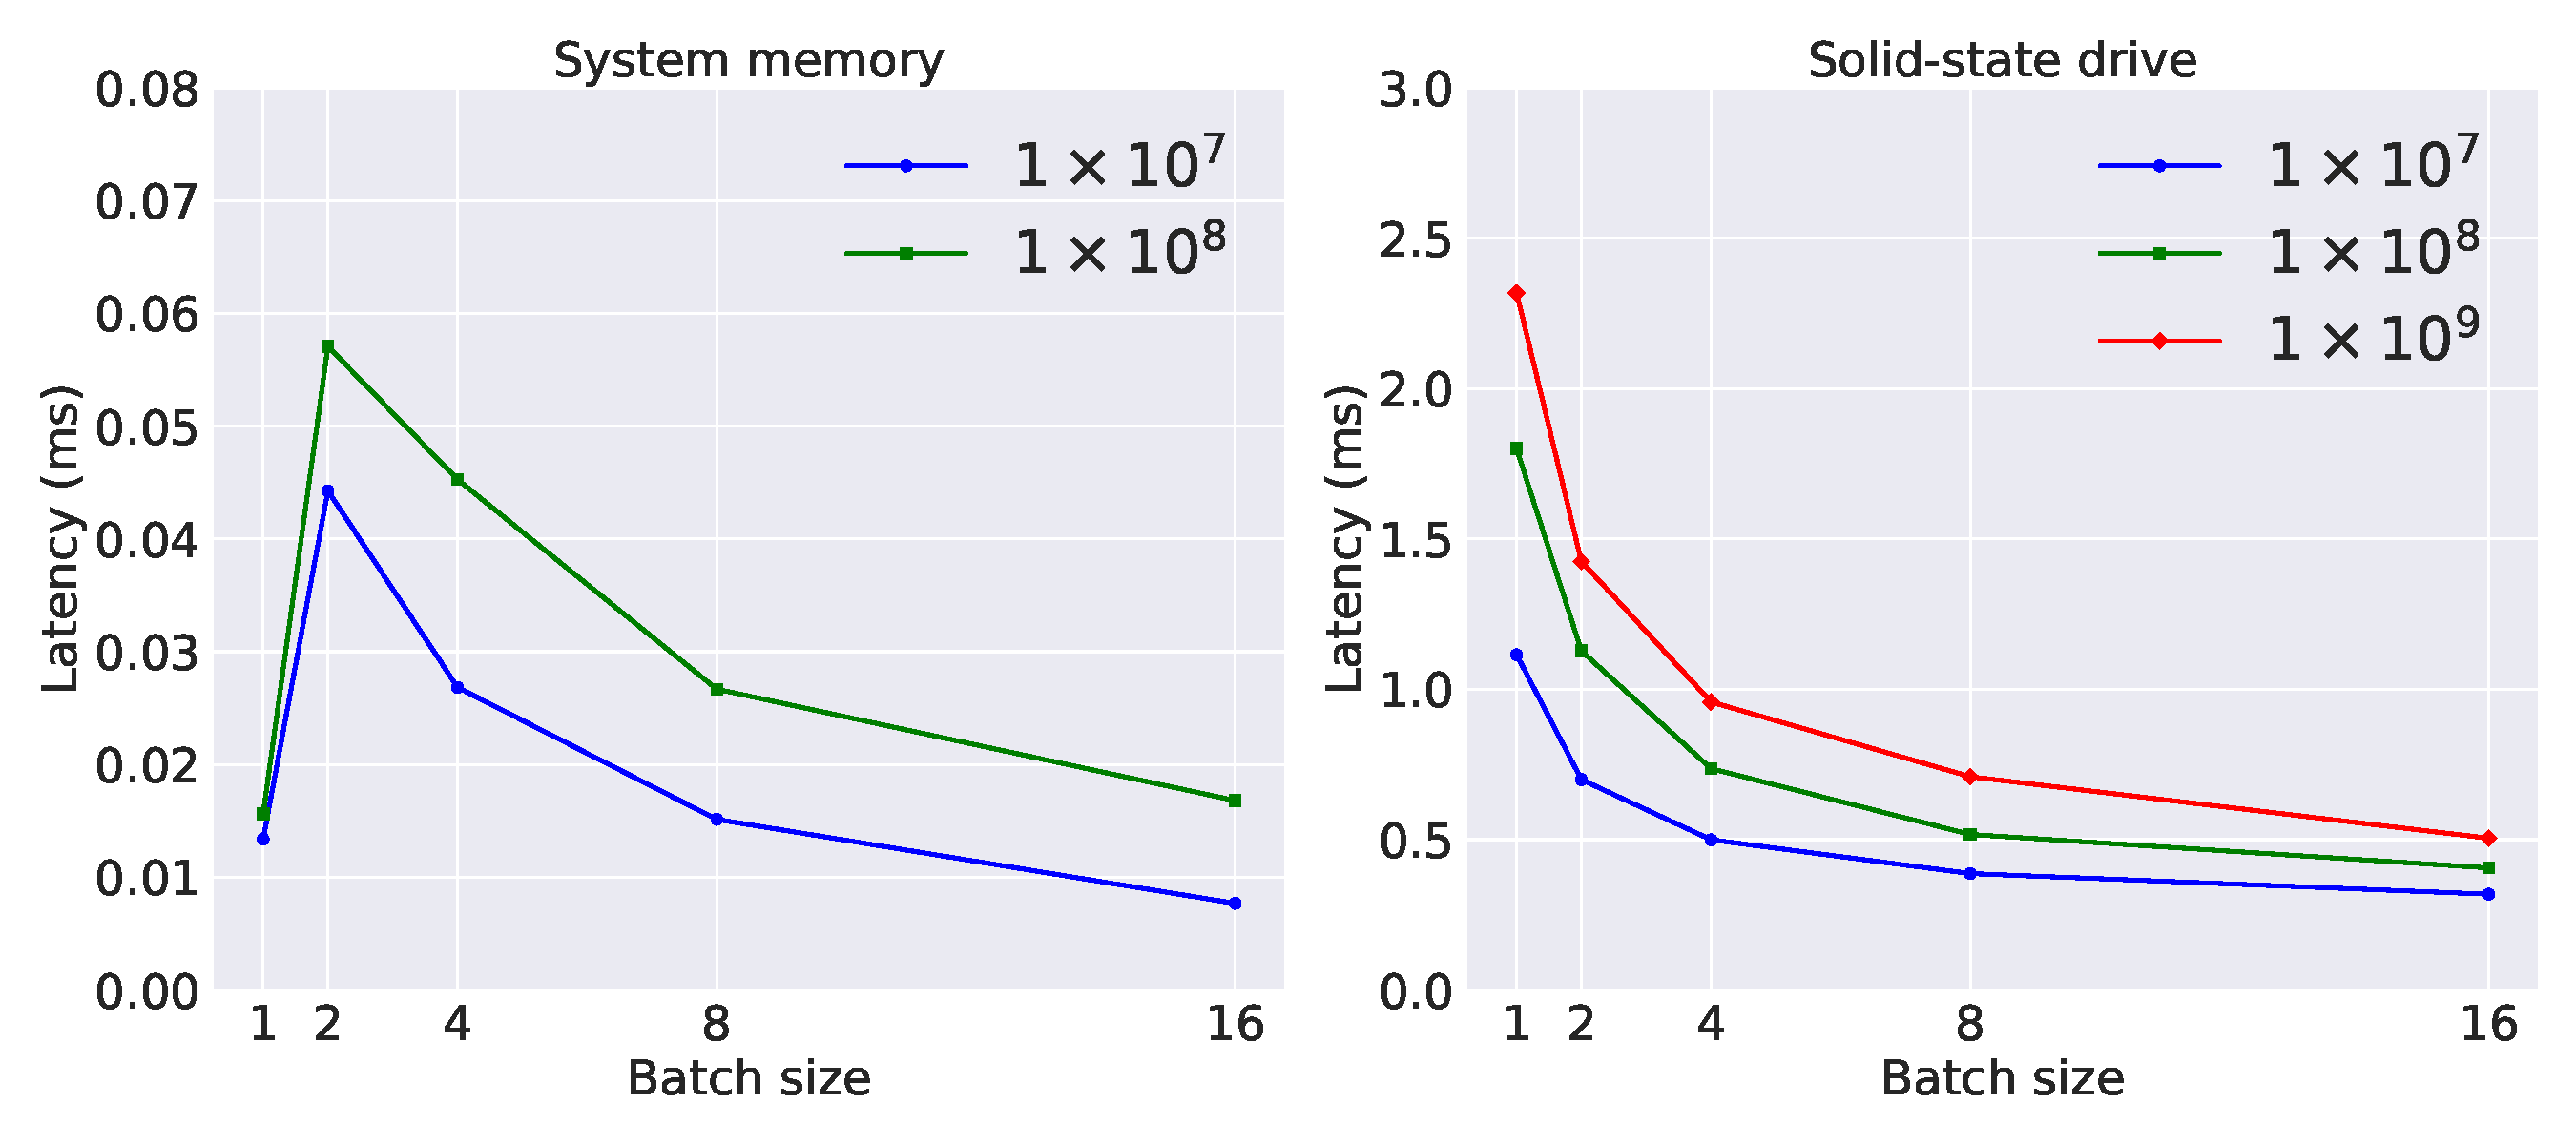
\includegraphics[width=0.8\linewidth]{figs/olmo_query_latency.pdf}
    \caption{Amortized per-token query latency (ms), averaged over 100,000 batches. The latency spike from batch size 1 to 2 when reading from system memory is due to batch operator overhead, which is less pronounced for solid-state drives. }

    \label{fig:latency}
\end{figure}

\Cref{fig:latency} shows the latency of retrieving embeddings at different batch sizes. Latency is measured as the end-to-end time from loading a batch of tokens to having the f-gram embeddings ready on the GPU.
Before each test, the CPU cache is cleared. Up to four queries per token are performed to find the longest matching \ngram{n} (for a maximum \ngram{n} length of $K=5$). For in-memory storage, sequential queries are sufficient since they are not the bottleneck, whereas on-disk storage uses parallel queries to the database.
At a batch size of 1, retrieval from a 10M f-gram embedding layer on NVMe takes 1.1 ms, increasing to 2.3 ms for a 1B-layer: both well below the latency threshold for LLM inference (typical commercial APIs generate at $\sim$100 tokens/sec, or $\sim$10 ms/token \citep{generation_speed}).
Larger batch sizes further improve efficiency: at batch size 16, amortized per-token latency drops to 0.5 ms. In-memory access is much faster: for a 100M f-gram layer at batch size 16, per-token latency is only 0.017 ms.
We also report end-to-end generation speed in \Cref{fig:olmo_scaling_result}, which aligns with these latency trends: when embeddings are stored in main memory, there is negligible impact on throughput; when stored on NVMe drives, throughput slightly decreases but no major bottleneck arises.
